\documentclass{article}

\usepackage[version=3]{mhchem} % Package for chemical equation typesetting
\usepackage{siunitx} % Provides the \SI{}{} and \si{} command for typesetting SI units
\usepackage{graphicx} % Required for the inclusion of images
\usepackage{natbib} % Required to change bibliography style to APA
\usepackage{amsmath} % Required for some math elements 

\setlength\parindent{0pt} % Removes all indentation from paragraphs

\renewcommand{\labelenumi}{\alph{enumi}.} % Make numbering in the enumerate environment by letter rather than number (e.g. section 6)

%\usepackage{times} % Uncomment to use the Times New Roman font
\usepackage{hyperref}
\usepackage{listings}


%----------------------------------------------------------------------------------------
%	DOCUMENT INFORMATION
%----------------------------------------------------------------------------------------
\title{Programming of Supercomputers \\ Assignment 1 Report} % Title
\author{Denys \textsc{Sobchyshak} and Denys \textsc{Korzh}} % Author name
\date{\today} % Date for the report

\begin{document}
\maketitle % Insert the title, author and date

%----------------------------------------------------------------------------------------
%	SECTION 1
%----------------------------------------------------------------------------------------
\section{Description and objectives}
In this assignment we focused greatly on single core optimization as this aspect tends to receive only a minor attention during the optimization stages of projects and took a look at possible I/O performance fine-tuning, which is quite important when dealing with vast amounts of data. As a basis we used AVL FIRE\textregistered\ benchmark, which is a 2D or 3D simulation of flow and heat transfer within arbitrary complex geometries with moving or fixed boundaries. As a result of our analysis we wanted to see how different optimization techniques relate to each other and what potential benefits our simulation code might get.

\section{Execution environment}
Measurements are being carried out on a SuperMUC thin node with a PAPI version 5.1.1.0. We allocate one full node for our job even though we require just one core for the task because it is not possible to allocate less compute power. To perform the actual computation and event collection we are using a batch script that triggers our binary as follows:

\begin{lstlisting}[frame=single]
#!/bin/bash
#@ job_name = pos_ws1_papi
#@ job_type = parallel
#@ class = test
#@ island_count=1
#@ node = 1
#@ total_tasks=16
#@ wall_clock_limit = 0:30:00
#@ energy_policy_tag = pos_ws1_papi_tag

#@ initialdir = $(home)
#@ output = $(home)/job-vec.out
#@ error = $(home)/job-vec.err

#@ queue

#system setup
perf_off

#job triggering code here
./gccg ./data/cojack.dat -cache
\end{lstlisting}
Detailed description of the execution environment can be found in the submitted archive in A1/data/supermuc-stats.ods.
 
%----------------------------------------------------------------------------------------
%	SECTION 2
%----------------------------------------------------------------------------------------
\section{Sequential optimization analysis}

\subsection{Performance measurements using PAPI}
In order to collect the data following PAPI counter events were used:\\
\begin{center}
\begin{tabular}{l|c}
	\hline
	Event & Description \\
	\hline
	PAPI\_DP\_OPS & Floating point operations; optimized to count vector operations \\
	PAPI\_L2\_TCM & Level 2 cache misses \\
	PAPI\_L2\_TCA & Level 2 total cache accesses \\
	PAPI\_L3\_TCM & Level 3 cache misses \\
	PAPI\_L3\_TCA & Level 3 total cache accesses \\
\end{tabular}
\end{center}
and consequently the next formulas to compute metrics were used:
\begin{center}
	$MFLOPS=\frac{PAPI\_FP\_OPS}{end\_time\_usec - start\_time\_usec}$
\end{center}
\begin{center}
	$L2\_CACHE\_MISS\_RATE=\frac{PAPI\_L2\_TCM}{PAPI\_L2\_TCA}*100$
\end{center}
\begin{center}
	$L3\_CACHE\_MISS\_RATE=\frac{PAPI\_L3\_TCM}{PAPI\_L3\_TCA}*100$
\end{center}
where end\_time\_usec and start\_time\_usec are corresponding PAPI start and end time values.

\subparagraph{Execution time}
As we carried out our measurement experiemnts on the SuperMUC we observed that runtime of the computational phase decreased by roughly 23\% once we used -O3 flag. This behaviour is true for both files and makes sence, since the latter optimization flag enables agressive loop optimizations for speed while the former one just carries out code size optimizations. Please see runtime graph on figure \ref{fig:1}.
\begin{figure}[h]
	\begin{center}
		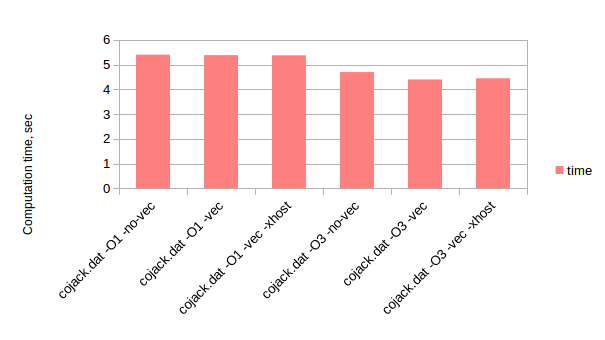
\includegraphics[width=0.8\textwidth]{comp-time} % Include the image placeholder.png
		\caption{Comparison of computational time}
		\label{fig:1}
	\end{center}
\end{figure}

\subparagraph{Cache miss rates}
The cache miss rates for both L2 and L3 caches increased by a rough 22\%. In general this can be explained by adressing the fact that -O3 flag employes vectorization, which means that our program will load all the data at once instead of making numerous load calls, which reduces the total number of memory loads. However, every time that the program would access a cache line in a way that predictor didn't anticipate it will cause a cache miss. Which means that the total numer of loads decreases while approximately the same number of cache lines are being touched. Comparison of cache miss rates can be found on figure \ref{fig:2}.
\begin{figure}[h]
	\begin{center}
		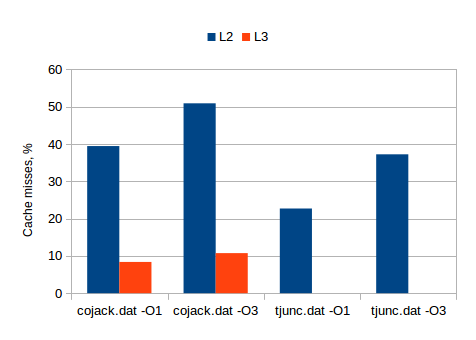
\includegraphics[width=0.8\textwidth]{cache-misses} % Include the image placeholder.png
		\caption{Comparison of cache misses}
		\label{fig:2}
	\end{center}
\end{figure}

\subparagraph{MFLOPS counters}
In addition, we observed that once -O3 flag was employed measured MLUPS increased only marginally. Analysis of such a delicate matter is hard to perform with raw instruments, however it is known that optimization might include various techniques like excluding common calculations out of loops, pre-calculating expressions, fusing constants and so on which will decrease the number of operations performed while the actual runtime might not decrease substantially. Also, measurement of FLOP in modern architectures is not a very straightforward task and requires more elaborate approach than the employed one. As of today, particularly for highly optimized code like the one we get via -O3 flag no single PAPI counter is likely to capture all floating point operations. A more detailed discussion of the matter can be seen \href{http://icl.cs.utk.edu/projects/papi/wiki/PAPITopics:SandyFlops}{here}. Furthermore, while comparing with the peak system performance of ~21.6 thousand MFLOPS we can see that computing data for our biggest problem set cojack.dat is performed at ~7 thousand MFLOPS which is roughly 32\% of the possible performance.

\subsection{Effect of vectorization}
While carrying out measurements of vectorized versus novectorised banchmark runtime under different optimization options we have observed that there is virtually no change in runtime for -O1 optimization flag, which is expected since -O1 flag doesn't use auto-vectorization optimizations, however with -O3 flag we have noticed a slight changes in runtime. Specifically, enabled vectorization versus diabled one decreases the runtime of simulation by roughly 7\%. Such behaviour can be explained by the fact that in the computation code 11 loops were vectorized.Vectorization report suggested that more optimization can be carried out, however, it has to be checked whether such optimization will improve performance or not. Besides using -O3 enabled high level loop optimizations which might make it easier for the compiler to vectorise the resulting code. Furthermore, we measured computation time while having -xhost flag enabled and it slows down the simulation by around 1.2\%. This is most likely observed because vectorization can sometimes slow execution due to pipeline synchronization, data movement timing or other issues.

%----------------------------------------------------------------------------------------
%	SECTION 3
%----------------------------------------------------------------------------------------
\section{I/O performance analysis}
After comparing input file sizes and the time it takes to load them we have noticed a drastic fall in both processing time and binary file sizes. This is an expected behaviour since text files are basically binary files that store ASCII codes. In particular, it means that for each and every decimal, for example, a text file will store far more than 8 bytes, unlike the binary file. Thus size of a file containing less bytes will be smaller, which is the case with binary files. Furthermore, since in order to read text files a program needs to first read ASCII codes and then convert them, it takes more processing time to read a text file. Visualized comparison of loading times and file sizes is shown on figure \ref{fig:3}.

\begin{figure}[h]
\begin{center}
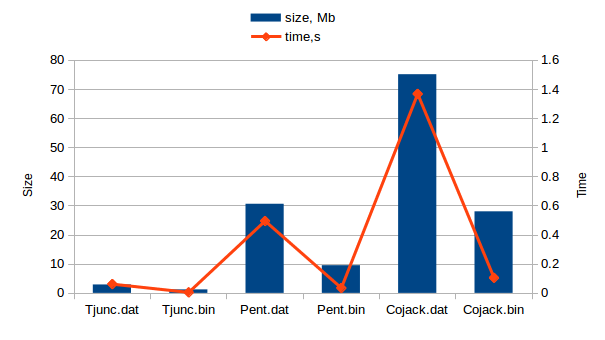
\includegraphics[width=0.8\textwidth]{time-size} % Include the image placeholder.png
\caption{Comparison of file sizes and their read times}
\label{fig:3}
\end{center}
\end{figure}
%----------------------------------------------------------------------------------------
\end{document}